%%====================%%
%%  Part III Project  %%
%%====================%%

\documentclass[aps,prd,reprint,preprintnumbers,showpacs,floatfix,nofootinbib,superscript address]{revtex4-2}
\usepackage[utf8]{inputenc}
\usepackage{parskip}
\usepackage{amssymb}
\usepackage{stix}
\usepackage{hhline}
\usepackage{amsmath}
\usepackage{mathtools}
\usepackage[dvipsnames]{xcolor}
\usepackage{xspace}
\usepackage{multirow,tabularx}
\usepackage{siunitx}
\usepackage{multirow}
\usepackage{graphicx}
\usepackage{xstring}
\usepackage{etoolbox}
\usepackage{notoccite}
\usepackage{natbib}
\usepackage{mathrsfs}
\usepackage{lineno}
\usepackage{tensor}
\usepackage{accents}
\usepackage{tikz}
\usepackage{listings}
\allowdisplaybreaks
\parskip 1mm
\parindent 2mm

%%===========================%%
%%  Part III Project Macros  %%
%%===========================%%

%	The Planck mass
\newrobustcmd{\Planck}{%
	{M_{\text{Pl}}}%
}

%	The Riemannian covariant derivative
\newrobustcmd{\rD}[1]{%
	\tensor{\mathring{\nabla}}{#1}%
}

%	The Riemann-Cartan covariant derivative
\newrobustcmd{\rcD}[1]{%
	\tensor{\nabla}{#1}%
}

%	The Riemann tensor
\newrobustcmd{\rR}[1]{%
	\tensor{\mathring{R}}{#1}%
}

%	The Riemann-Cartan tensor
\newrobustcmd{\rcR}[1]{%
	\tensor{R}{#1}%
}

%	Irreducible parts of the torsion
\newrobustcmd{\T}[2][placeholder]{%
	\IfEqCase{#1}{%
	{placeholder}{\tensor{T}{#2}}%
	{1}{\tensor[^{(1)}]{T}{#2}}%
	{2}{\tensor[^{(2)}]{T}{#2}}%
	{3}{\tensor[^{(3)}]{T}{#2}}%
	}%
	[\packageError{cosmicclass}{Symbol #1 is not an irreducible part!}{}]%
}

%	Irreducible parts of the multiplier
\newrobustcmd{\TLambda}[2][placeholder]{%
	\IfEqCase{#1}{%
	{placeholder}{\tensor{\lambda}{#2}}%
	{1}{\tensor[^{(1)}]{\lambda}{#2}}%
	{2}{\tensor[^{(2)}]{\lambda}{#2}}%
	{3}{\tensor[^{(3)}]{\lambda}{#2}}%
	}%
	[\packageError{cosmicclass}{Symbol #1 is not an irreducible part!}{}]%
}
 %some personal macros

\usepackage{hyperref}
\hypersetup{%
     colorlinks = true,%
     linkcolor = Blue,%
     citecolor = Blue,%
     filecolor = Blue,%
     urlcolor = Blue% 
     }%
\usepackage[capitalize]{cleveref} %always load this last in preamble

\newcommand{\signature}[2][8em]{%
  \begin{tabular}[t]{ p{#1} p{#1} }
    \strut\raggedleft
    \raisebox{-.5ex}[0pt][0pt]{\bfseries #2} & \\
    \cline{2-2}
    & \centering\scriptsize\itshape (signature)
  \end{tabular}
}

\usepackage[style=nejm, 
citestyle=numeric-comp,
sorting=none]{biblatex}
\addbibresource{Bibliography.bib}


\nocite{*}

\begin{document}

\title{Constraints on inflation from scale-invariant gravity}

\author{Prabhoda CS}
\affiliation{Department of Physics, Cavendish Laboratory, University of Cambridge}

\begin{abstract}
This following document maps the road plan for the part III project `Constraints on inflation from scale-invariant gravity' illustrating what was done and what is the end goal of the project. We start with a short summary of the literature reviewed to familiarize the reader with the basics such as what is cosmic inflation, why it is posited and it's mechanism of action. We then talk about the specifics of the inflationary model being considered here in this project. 

The progress so far and the goals of the project are then discussed in the final section of the document

\end{abstract}

\maketitle


\section{The need for Inflation}\label{The need for Inflation}

\indent The simplest model of the Big Bang theory naturally follows from General Relativity applied to a general isotropic and homogeneous universe (Friedmann Equations) combined with Hubble's observations (Hubble's Law). This theory describes a universe with a constant expansion rate. It is a highly successful theory, able to offer a comprehensive explanation for a lot of experimental observations such as the CMB, the abundance of light elements, large scale structure and mainly, Hubble's Law.

However, there are several problems with this simple model. In the following section, we will present two arguments against the conventional Big Bang theory.

\subsection{Horizon Problem}
In this section, we will show that given the standard assumed expansion rate in the big bang model, we cannot satisfactorily explain the near-perfect uniformity of the CMB. This is because, given the rate of expansion, there is no way for distant regions of the CMB to have once been causally connected.
Given the Friedmann Equations and defining the Hubble constant $H = \frac{\dot{a}}{a}$,
\begin{equation} \label{1}
    \dot{\rho} = -3(\rho + p)H
\end{equation}
\begin{equation} \label{2}
    \Ddot{a} = -\frac{4\pi G}{3} (\rho + 3p)a
\end{equation}
\begin{equation}    \label{3}
    H^2 + \frac{k}{a^2} = \frac{8 \pi G}{3} \rho
\end{equation}

From the continuity equation \ref{1}, we have:
\begin{equation} \label{4}
    \frac{\mathrm{d}  \ln(\rho)}{\mathrm{d} \ln(a)} = -3(1+w)
\end{equation}

Where, $w = \frac{p}{\rho}$. We can solve this equation to get $\rho \propto a^{-3(1+w)}$. In combination with Friedmann equation \ref{3} for a flat universe $k = 0$, we get the scale factor $a$ as a function of time $a(t)$.

\begin{equation}    \label{5}
    a(t) = \begin{cases}
        t^{2/3(1+w)} & w \neq -1 \\
        e^{Ht} & w = -1
    \end{cases}
\end{equation}

Now, we can define the comoving horizon ($\tau$) as the causal horizon or the maximum distance a light ray can travel between times 0 and $t$.

\begin{equation}    \label{6}
    \tau \equiv \int_{0}^{t} \frac{\mathrm{d} t'}{a(t')} = \int_{0}^{a} \frac{\mathrm{d}a}{H a^2} = \int_{0}^{a} \mathrm{d} \ln(a) \frac{1}{aH}
\end{equation}

For a conventional Big Bang model, therefore, the causal horizon $\tau$ for a universe with $w \geq 0$ increases with time. In plain words, this means that the fraction of the universe with each other increases with time.
\begin{equation}
    \tau \propto a^{1/2(1+3w)} \implies \tau = \begin{cases}
        a & \text{Radiation Dominated} \\
        a^{1/2} & \text{Matter Dominated}
    \end{cases}
\end{equation}

The comoving horizon increasing with time implies that comoving scales (comoving scale is not the same as the physical scale) entering the cosmic horizon now were not in causal contact during the CMB decoupling! However, the anisotropy of the CMB is about one part in $10^{-5}$, posing a problem to the conventional big bang model to explain how these distant regions of the CMB managed to regulate their temperatures to such an accurate degree.

\subsection{Flatness Problem}
We know that despite the presence of mass and energy in our universe, the large scale structure of out spacetime is approximately Euclidean (flat). To see whether this is a stable equilibrium, we return to Friedmann equation \ref{3} and defining $\rho_{\text{crit}} = 3H^2(a)$ and $\Omega(a) = \frac{\rho(a)}{\rho_{\text{crit}}}$, we get
\begin{equation}
    1 - \Omega(a) = \frac{-k}{(aH)^2}
\end{equation}
Differentiating this equation and using the Friedmann equations, we get,
\begin{equation}
    \frac{\mathrm{d}\Omega}{\mathrm{d} \ln a} = (1+3w)\Omega(\Omega-1)
\end{equation}
Looking at this, we can see that $\Omega = 1  \implies \rho = \rho_{crit}$ is an unstable equilibrium and slight perturbations can make the universe not flat i.e., $k \neq 0$. This means that in the standard big bang model, matter density has to be extremely fine tuned to fit the requirement $\rho = \rho_{crit}$, which seems unlikely.

The theory of inflation attempts to resolve the need for extreme fine tuning of the initial conditions of the universe by positing a period of exponential expansion. The next section shows how this theory solves the two problems stated above.

\section{Inflation}\label{Inflation}

Looking at both the problems highlighted in the previous section, we see that the comoving Hubble radius ($(aH)^{-1}$) plays an important role
\begin{equation}    \label{10}
    \tau = \int_{0}^{a} \mathrm{d} \ln (a) \frac{1}{aH}
\end{equation}
\begin{equation} \label{11}
    1 - \Omega (a) = \frac{-k}{(aH)^2}
\end{equation}
If the comoving Hubble radius was decreasing, this means that large scales entering the present universe were inside the horizon before inflation. By equation \ref{11}, it also means that $\rho = \rho_{crit}$ is a stable equilibrium as the solution $\Omega = 1$ is an attractor during inflation.

A decreasing comoving horizon directly implies a period of accelerated expansion as seen by taking it's derivative
\begin{equation}
    \frac{\mathrm{d}}{\mathrm{d}t} \frac{1}{aH} <  0 \implies \frac{-\Ddot{a}}{(aH)^2} < 0 \implies \ddot{a} > 0
\end{equation}
Given that $\ddot{a} > 0$ and Friedmann equation \ref{2}, we see that $\frac{\rho}{3} < p \implies w < - \frac{1}{3}$. This is a violation of the strong energy condition.

So far, we have described the physical implications of inflation and it's effects. In the following section, we shall describe the physical conditions under which such an exponential expansion can arise. 

\subsection{Scalar Field Inflation}
The simplest models of inflation involve a scalar field $\phi$ (Inflation Field) that acts as the perfect fluid with $w < -\frac{1}{3}$ such that upon coupling with gravity through the Einstein-Hilbert action, it can provide the repulsive force in the Friedmann equations for the accelerated expansion.

The dynamics of a scalar field minimally coupled to gravity is governed by the action

\begin{equation}
    S = \int \mathrm{d}^4 x \sqrt{-g} \left[ \frac{1}{2} R + g^{\mu \nu}\partial_{\mu}\phi \partial_{\nu} \phi  - V(\phi) \right] = S_{\text{EH}} + S_{\phi}
\end{equation}
Using Noether's Theorem, we see that the energy momentum tensor for the scalar field gives,
\begin{equation}
    T_{\mu \nu} = \partial_{\mu} \phi \partial_{\nu} \phi - g_{\mu \nu} \left( \frac{1}{2}\partial_{\sigma} \phi \partial^{\sigma}\phi - V(\phi) \right)
\end{equation}
Using the energy momentum tensor and assuming homogeneity in the perfect fluid (scalar field), we get
\begin{equation}
    \rho_{\phi} = \frac{1}{2}{\dot{\phi}}^2 + V(\phi)
\end{equation}
\begin{equation}
    p_{\phi} = \frac{1}{2}{\dot{\phi}}^2 - V(\phi)    
\end{equation}

Substituting these values of $\rho$ and p into the continuity equation \ref{1} and also using equation \ref{3} and substituting $k = 0$, we get 

\begin{equation} \label{17}
    \ddot{\phi} + 3H\dot{\phi} + V,_\phi = 0
\end{equation}

\begin{equation} \label{18}
    H^2 = \frac{8\pi G}{3} \left(\frac{1}{2} {\dot{\phi}}^2 + V(\phi) \right)
\end{equation}

\subsection{Slow Roll Inflation}
The acceleration equation for universe dominated by the inflaton field with the energy density $\rho_{\phi}$ and pressure $p_{\phi}$ is given by Friedmann equation \ref{2},
\begin{equation}
    \frac{\ddot{a}}{a} = -\frac{4\pi G}{3} (\rho +3p) = -\frac{8\pi G}{3} ({\dot{\phi}}^2 - V(\phi)) 
\end{equation}
We see that if we can get $\ddot{a} > 0$ by requiring $\dot{\phi}^2 << |V(\phi)|$. This period is called slow roll because when this condition is satisfied, it corresponds to the scalar field slowly rolling down it's potential hill. The accelerated expansion will also only be satisfied for a long period of time if we require $|\ddot{\phi}| << 3H\dot{\phi} \sim |V,_{\phi}|$. 

We can rewrite these two slow-roll conditions with the two slow roll parameters $\epsilon$ and $\eta$ and requiring that $\epsilon << 1$ and $\eta << 1$ during the slow roll. 
\begin{equation}
    \epsilon = \frac{1}{2}  \left( \frac{V,_{\phi}}{V} \right)^2 \,\,\,\,\,\,\,\,\ \eta = \left| \frac{V,_{\phi\phi}}{V} \right|
\end{equation}

With these conditions in place, the two equations relating the scale factor and the scalar field \ref{17} and \ref{18} reduce to
\begin{equation}  \label{21}
    3H\dot{\phi} + V,_{\phi} = 0 \,\,\,\,\,\,\,\,\,\,\,\  H^2 = \frac{8\pi G}{3} V(\phi)
\end{equation}

So far, these arguments only provide restrictions on the potential of the scalar field $\phi$, but make no attempt to motivate the form of the potential or the action principle for the field from first principles. This is inflation refers to a whole host of theories which aim to explain the mechanism behind the period of exponential expansion that occurred when the universe was around $\geq 10^{-34}s$ old.

One of the ways to arrive at the action principle of the inflaton field is to take a leaf out of the playbook of many successful QFTs and to hypothesize a gauge condition. This is the approach that shall be taken in this project and explained more in the next section.


\section{Scale Invariant Gravity} \label{Section 3}
Having laid the groundwork, we now come to the primary study of this project. This is based on the paper \cite{barker2024poincaregaugetheoryconformal} mainly and will follow up on the idea and look at it's conclusions. 

The theory of General Relativity is one of mankind's most rigorous scientific theories, is self consistent and so far, all tests of GR have been shown to be in agreement with the theory. However, we do not \textit{a priori} know that the theory of general relativity can be extended to arbitrary energy (/length) scales. It is widely accepted that at high enough energy scales, those comparable to the planck scale, GR breaks down. 

An interesting possibility to consider is that GR as we know it, with the Einstein-Hilbert lagrangian being proportional to the Ricci Scalar, is a low energy extrapolation of a more fundamental scale invariant theory which describes physics at higher energies. 

Let us begin by exploring this possibility with a simple spin-0 scalar field that is minimally coupled to gravity.

\begin{equation}
    S = \int \mathrm{d}^4 x \sqrt{-g} \frac{1}{2} \left[ \partial_\mu \varphi \partial^\mu \varphi - m^2   \varphi^2   \right] + \text{gravity}
\end{equation}

Before we can require global scale invariance in the theory, we immediately see that there is a problem. Looking at the dimensions of the terms, ($[\partial_\mu \varphi \partial^\mu \varphi ] = 4$) and ($[\varphi^2 ] = 2$) (In natural units).  For such a transformation to leave the action invariant, we would want all the terms in the action to transform similarly, however, while the first term of the action transforms with 4 powers of the transformation the second term only transforms with 2 powers, due to it's dimension. The only way to fix this is to make $m$ a dynamic field $\phi$  and couple it with $\varphi$ using a dimensionless coupling parameter $\mu$.

\begin{subequations}\label{23}
\begin{align}
    S = \int \mathrm{d}^4 x \sqrt{-g} \bigg[ &\frac{1}{2} \Big( \partial_\mu \varphi \partial^\mu \varphi + \sigma \partial_\mu \varphi \partial^\mu \phi \nonumber\\
    &+ \nu \partial_\mu \phi \partial^\mu \phi - \mu^2 \phi^2 \varphi^2 \Big) \bigg] + \text{gravity}.
\end{align}
\end{subequations}

We can now gauge this scale invariance (make the transformation local) to see what the resulting dynamics entail. Under local scale invariance, the metric transform as $g_{\mu \nu} \rightarrow e^{2\rho} g_{\mu \nu}$ and the scalar fields as $\varphi \rightarrow e^{-2\rho} \varphi$ and $\phi \rightarrow e^{-2\rho} \phi$, where $\rho = \rho(x)$. To ensure that the derivative terms respect this transformation, however, we are forced to introduce a vector potential term in a similar vein to QED, which transforms as such $B_{\mu} \rightarrow B_{\mu} - \partial_{\mu}\rho$.

This new field however, cannot propagate on it's own, if we want there to be only degree of freedom between the fields $\varphi$ and $\phi$, we need to choose a suitable gauge. One choice is the Einstein gauge $\phi = \phi_{0}$, however, we can also redefine away the field $\phi$, by choosing $g_{\mu \nu} \rightarrow \frac{\phi_0}{\phi} g_{\mu \nu}$, $\varphi \rightarrow \frac{\phi}{\phi_0} \varphi$ and $B_{\mu} \rightarrow B_{\mu} - \partial_{\mu} ln(\phi)$. Putting all this together, we get

\begin{widetext}
\begin{subequations}
\begin{align}\label{24}
    S = \int \mathrm{d}^4 x \sqrt{-g} \left[ \frac{1}{2}  (\partial_\mu \varphi - (\varphi - \sigma \phi_0)B_\mu)(\partial^\mu \varphi - \varphi B^\mu)  - 
    \frac{\mu^2\phi_{0}^{2}}{2} \varphi^2 - \frac{\xi}{16} H_{\mu\nu}H^{\mu\nu} + \frac{\nu \phi_{0}^{2}}{2} B_\mu B^\mu \right] + \text{gravity}
\end{align}
\end{subequations}
\end{widetext}

We are left with a slight problem here, while we set out to discover the dynamics of the inflaton field $\varphi$, we have two fields here, one scalar $\varphi$ and another vector field $B^\mu$. Given that there is no need for an additional vector particle in either particle physics or cosmology, we can employ a trick of sending $\nu \rightarrow \infty$, this has the effect of making the particle heavy and could be seen as a dark matter candidate. For sufficiently large $\nu$, we can ignore the $H_{\mu\nu}H^{\mu\nu}$ term and solve for $B^\mu$ using the Euler-Lagrange equations and get $B^\mu = \frac{1}{2} \partial^\mu \text{ln}(\varphi^2 - \sigma \phi_0 \varphi + \nu \phi^2)$. Substituting this into \ref{24}, we get

\begin{equation}
    S = \int \mathrm{d}^4 x \sqrt{-g} \frac{1}{2} \left[ \partial_\mu \varphi \partial^\mu \varphi - U(\varphi)   \right] + \text{gravity}
\end{equation}
where
\begin{equation} \label{26}
    U(\varphi) = \frac{\mu^2 \phi_{0}^{4}}{2} \left[ \frac{\sigma}{2} + \sqrt{\nu - \frac{\sigma^2}{4}} \text{sinh}\left( \frac{\varphi - c}{\phi_0 \sqrt{\nu - \frac{\sigma^2}{4}}} \right)  \right]
\end{equation}

We can see the graph of the potential in Fig \ref{Potential from Paper}.
\begin{figure}[h]
    \centering
    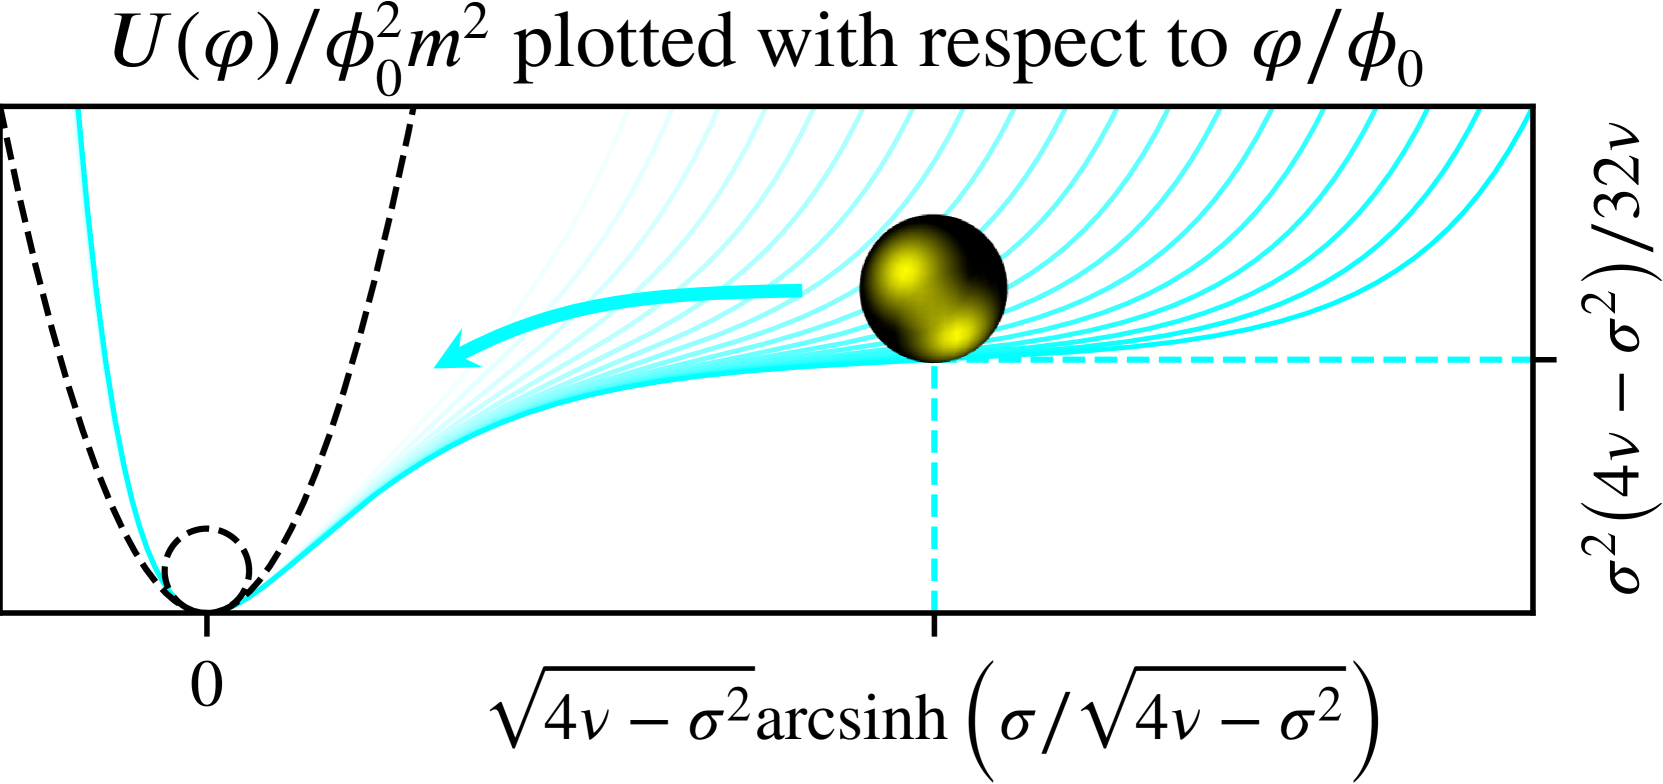
\includegraphics[width=0.5\textwidth]{Potential from Paper.png}
    \caption{Graph of the potential \cite{barker2024poincaregaugetheoryconformal}}
    \label{Potential from Paper}
\end{figure}


\section{Project Plan}

\subsection{Work Done}

In the first two weeks of the project, I reviewed the literature on the topic \cite{Mukhanov:2005sc}, \cite{baumann2012tasilecturesinflation}. This was to familiarize myself with the topics of cosmic inflation and the tools used to describe it. 

Upon getting a handle on the tools required, in week 3 and 4, I referred to the papers \cite{barker2024poincaregaugetheoryconformal} and \cite{Salvio_2022} to understand the derivation of the specific potential as described in section \ref{Section 3}. I also translated the equations to code and propagated the field to see how it would look.

To do this, the potential $U(\varphi)$ from section \ref{Section 3} equation \ref{26} was used in the equations \ref{21} to get a differential equation for the field $\varphi$. We also use the following relation to calculate the number of e-folds during inflation valid in the slow roll region,
\begin{equation}
    N(\varphi) = \int_{\phi_\text{end}}^{\phi} \frac{V}{V,_{\phi}} \mathrm{d}\varphi
\end{equation}
to fix the parameters [$\mu,\phi_0,\sigma,\nu,c$] = [1, 1.5, 11, 50, 0] such as to get the $N \approx 50.131$.

To plot the functions in a more self-evident manner, we use the relation $\mathrm{d}N = H \mathrm{d}t$ relating the number of efolds to the time, to rewrite the scalar field equation \ref{17} in terms of derivatives with respect to the number of efolds.

\begin{align}
    \ddot{\phi} + 3H\dot{\phi} + V,_\phi &= 0 
    \\
    H \frac{\mathrm{d}}{\mathrm{d}N} \left(H \frac{\mathrm{d}\phi}{\mathrm{d}N} \right) + 3 H^2 \frac{\mathrm{d}\phi}{\mathrm{d}N} + \frac{\mathrm{d}V}{\mathrm{d}\phi} &= 0    
\end{align}

Using the relations given by the Friedmann Equations \ref{2} and \ref{3}, we can simplify the final equation as:

\begin{equation}
    \frac{\mathrm{d}^2\phi}{\mathrm{d}N^2} + 3 \frac{\mathrm{d}\phi}{\mathrm{d}N} - \frac{1}{2} \left( \frac{\mathrm{d}\phi}{\mathrm{d}N} \right)^3 + \left[ 3 - \frac{1}{2} \left( \frac{\mathrm{d}\phi}{\mathrm{d}N} \right)^2 \right] \frac{\mathrm{d}\text{ln}V}{\mathrm{d}\phi}  = 0
\end{equation}

The resulting graphs obtained given the parameters can be seen below. 

\begin{figure}[h!]
    \centering
    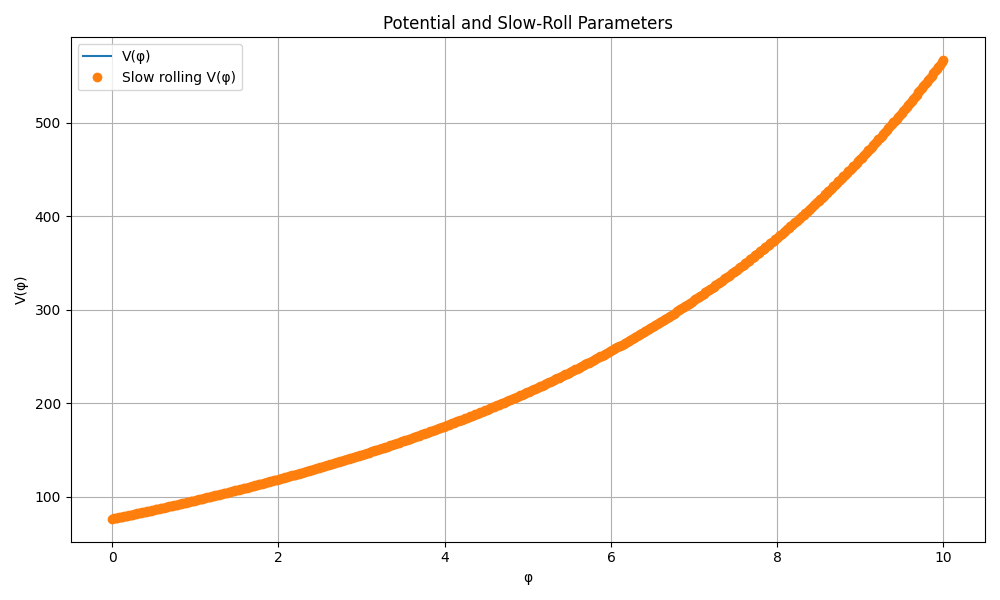
\includegraphics[width=0.4\textwidth]{Potential and Slow-Roll Parameters.png}
    \caption{Graph of the potential with the orange highlighting the slow roll region (Here, c = 8.41, to show the potential exiting slow roll)}
    \label{Potential as plotted by the code}
\end{figure}

\begin{figure}[h!]
    \centering
    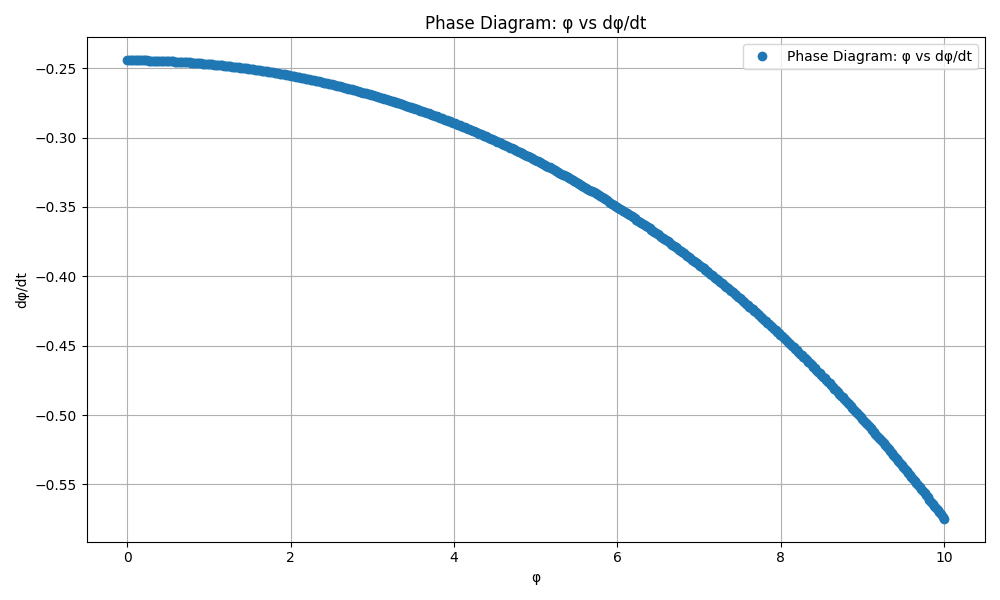
\includegraphics[width=0.4\textwidth]{Phase Diagram p vs dpdt.png}
    \caption{The phase diagram : $\dot{\varphi} \ \text{vs} \ \varphi$}
    \label{Phase Diagram}
\end{figure}

\begin{figure}[h!]
    \centering
    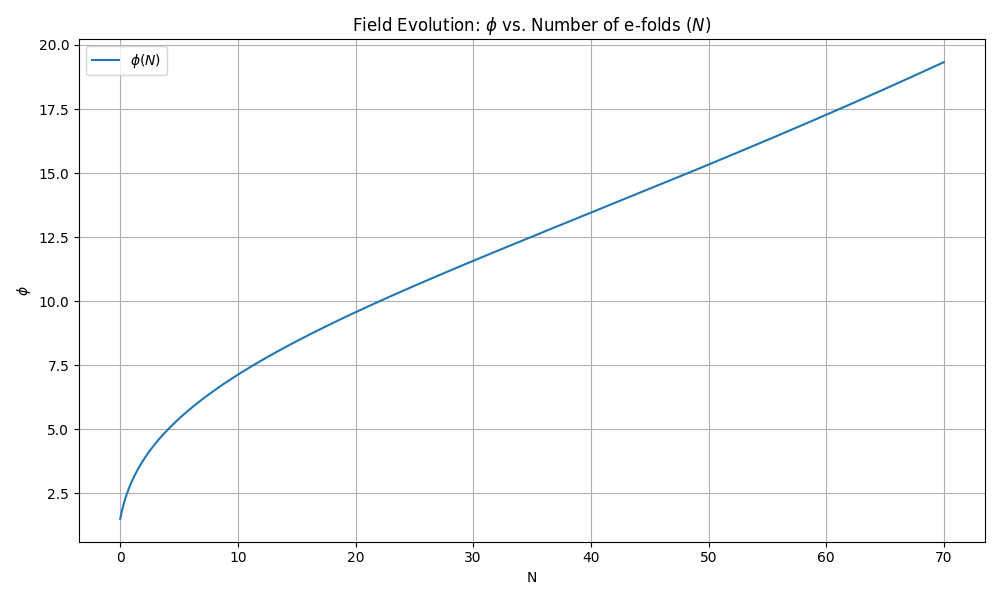
\includegraphics[width=0.4\textwidth]{Field as a function of N.png}
    \caption{The plot of the field $\varphi$ as a function of time $N$ (Number of efolds)}
    \label{Field as function of efolds}
\end{figure}

This code is available in the \href{https://github.com/PrabhodaCS/Part-III-Inflation-Project}{GitHub repo} to check.

\newpage

\subsection{Goal of the Project and Timeline}

The end goal of this project is to focus on the further theoretical development of this model, such as the addition of extra so-called "compensator" fields, and the resulting implications for the potential. Unusual features present in the potential which could give rise to non-standard power spectra could also be explored. 
\subsection{Timeline}
\begin{itemize}
    \item \textbf{CHRISTMAS BREAK} :
    Moving forward, I will have to re-review the paper \cite{Salvio_2022} and \cite{Blas_2011}, to see the alternative formulation taken to get to a similar looking potential as in \ref{26}. This formulation assumes the connection coefficients of GR to be independent of the metric (Unlike in GR, where the connection coefficients are the Christoffel symbols, are derived by assuming metric compatibility). This means that there are two independent parameters with respect to which the variation of the action can be taken, leading to different dynamics. The immediate next steps for me is to translate the variables used there to the ones used in this approach and show it's equivalence. We will also explore the power spectra predicted by the theory next. Read all necessary literature to prepare myself for the Lent and Easter terms.

    \item \textbf{LENT TERM}
    
    \begin{itemize}
        \item Weeks 1-2 : Add different compensator fields and check how the potential changes. Graphing the different potentials and looking at it's results.
        \item Weeks 3-4 : Look into paper \cite{Salvio_2022} and try to implement a combination of scalar inflaton fields and spacetime with torsion (Connection is non metric compatable). This will change the shape of the potential and will have different power spectra.
        \item Weeks 5-6 : Finalize models worth exploring further. Calculate power spectra of these different models.
        \item Weeks 7- 8 : Compare the models with the Planck data and analyse the parameter space and valid values of couplings. Prepare the main results of the paper.
    \end{itemize}

    \item  \textbf{EASTER TERM} Prepare the results of the paper. Compare different models and analyze literature to find similar end results. Analyze how perturbations in the model could result in the current CMB anisotropy. Look into different ways model could be extended and matched with experimental data. Prepare for VIVA and final project submission.
\end{itemize}



\vspace{5\baselineskip}

\mbox{}\hfill
\signature{Dr. Will Barker}\hfill
\mbox{}

\printbibliography

\end{document}
